\documentclass[12pt]{article}
\usepackage{graphicx}
\usepackage[margin=2cm, a4paper]{geometry}
\usepackage{setspace}
\usepackage{pdfpages}
\usepackage{float}
\usepackage{amsmath}
\usepackage{fancyvrb}
\usepackage{amssymb}
\usepackage{minted}
\usepackage{enumitem}
\usepackage{amsthm}
\usepackage[colorlinks,linkcolor=blue]{hyperref}


\renewcommand{\contentsname}{Contents}
\renewcommand{\figurename}{Figure}
\renewcommand{\tablename}{Table}
\hypersetup{
    colorlinks=true,
    linkcolor=black,
    filecolor=magenta,      
    urlcolor=blue,
}
\newcommand{\mytitle}{Probability Homework 4}
\newcommand{\myauthor}{B13902022 LAI, YU-CHI}

\usepackage{fancyhdr}
\pagestyle{fancy}
\fancyhead{}
\fancyhead[L]{\mytitle}
\fancyhead[R]{\myauthor}

\usepackage[english]{babel}
\newtheorem{theorem}{Theorem}[section]
\newtheorem{corollary}{Corollary}[theorem]
\newtheorem{lemma}[theorem]{Lemma}

\theoremstyle{definition}
\newtheorem{definition}{Definition}[section]
\theoremstyle{remark}
\newtheorem*{remark}{Remark}

\title{\mytitle}
\author{\myauthor}
\date{\today}

\begin{document}
\maketitle

\section*{3.2-17}
The pdf of chi-square distribution is:
$$f(x)=\frac{1}{\varGamma(r/2)2^{r/2}}x^{r/2-1}e^{-x/2}$$

In this problem $r=4$, so $f(x)=\frac{1}{4}xe^{-x/2}$. Let $X$ be the r.v. of $\chi^2(4)$.
\begin{align*}
    P(X>7.779)&=1-P(X\le 7.779) \\
    &=1-\int_{0}^{7.779}\frac{1}{4}xe^{-x/2}\mathrm{d}x \\
    &\approx 1-0.9=0.1
\end{align*}

Let $Y$ be the number of observations (out of 15) that exceeds $7.779$, since the observations are taken independently, it can be seen as a binomial distribution with $p=0.1, n=15$.
\begin{align*}
    P(Y\le 3)&=\sum^3_{k=0}\binom{15}{k}(0.1)^{k}(0.9)^{15-k} \\
    &=(0.9)^{15}+15\cdot (0.1)(0.9)^{14}+105\cdot (0.1)^2(0.9)^{13}+455\cdot (0.1)^3(0.9)^{12} \\
    &= 0.9444
\end{align*}

\fbox{Hence, the probability that at most 3 of the 15 observations exceed 7.779 is 0.9444.}


\newpage{}
\section*{3.2-18}
Let the r.v. $Y=X-80$, so $Y>0$ with pdf:
$$f(y)=\frac{y}{50^2}e^{-y/50},\ y>0$$

This is Gamma distribution with shape $\alpha=2$ and scale $\theta=50$.
\subsection*{(a)}
\begin{align*}
    \mu_{Y}=E[Y]=\alpha\theta=2\cdot 50=100 \\
    \mu_{X}=E[X]=E[Y+80]=E[Y]+80=180
\end{align*}
Shifting doesn't affect the variance:
$$\sigma^2_{X}=\sigma^2_{Y}=\alpha\theta^2=5000$$
\fbox{Hence, the mean is $180$ and the variance is 5000.}
\subsection*{(b)}
We can find the mode by setting $f'(y)=0$:
\begin{align*}
    f'(y)&=\frac{1}{2500}(e^{-y/50}-\frac{1}{50}ye^{-y/50}) \\
    &=\frac{1}{2500}e^{-y/50}(1-\frac{1}{50}y)=0 \\
    \Rightarrow\ y=50
\end{align*}
\fbox{Hence, the mode of $X$ is $50+80=130$.}
\subsection*{(c)}
This is equivalent to finding $P(Y<120)=1-P(Y\ge 120)$:
\begin{align*}
    P(Y<120)&=1-\int_{120}^{\infty}\frac{y}{50^2}e^{-y/50}\mathrm{d}y \\
    &=1-\frac{1}{2500}(-50ye^{-y/50}\mid^{\infty}_{120}+50\int_{120}^{\infty}e^{-y/50}\mathrm{d}y)\\
    &=0.6915
\end{align*}
\fbox{The percentage of having a serum cholesterol level less than 200 is 0.6915.}


\newpage{}
\section*{3.3-11}
We are given that $\mu=21.37,\sigma^2=0.16,\sigma=0.4$.
\subsection*{(a)}
Standardize using  $Z=\frac{X-\mu}{\sigma}$.
\begin{align*}
    P(X>22.07)=P(Z>1.75)=1-\Phi(1.75)=1-0.9599=0.0401
\end{align*}
where the value of $\Phi(1.75)$ is obtained by looking up the table.

\fbox{We obtained that $P(X>22.07)=0.0401$}

\subsection*{(b)}
\begin{align*}
    P(X<20.857)&=P(Z<-1.28) \\
    &=P(Z\le -1.28)+P(Z=1.28) \\
    &=[1-\Phi(1.28)]+\int_{1.28}^{1.28}f(x)\mathrm{d}x \\
    &=1-\Phi(1.28)=1-0.8997=0.1003
\end{align*}

Since each selection is independent, it can be seen as a binomial distribution with $p=0.1$ and $n=15$. ($Y$ is the r.v.)
\begin{align*}
    P(Y\le 2)&=P(Y=0)+P(Y=1)+P(Y=2) \\
    &= \binom{15}{0}(0.9)^{15}+\binom{15}{1}(0.1)(0.9)^{14}+\binom{15}{2}(0.1)^2(0.9)^{13} \\
    &=0.8159
\end{align*}
\fbox{So we have that $P(Y\le 2)=0.8159$.}

\newpage{}
\section*{4.1-9}
\subsection*{(a)}
For 15 independent items, $(X,Y,15-X-Y)$ follows a multinomial distribution. So the joint pmf is:
\begin{align*}
    f(x,y)=P(X=x,Y=y)=\frac{15!}{x!y!(15-x-y)!}(\frac{6}{10})^x(\frac{3}{10})^y(\frac{1}{10})^{15-x-y}
\end{align*}
And it's valid when $x\ge 0,y\ge 0,x+y\le 15$.
\subsection*{(b)}
By the constraints I previously mentioned, we can draw the following graph. (The colored region is the set of integers $(x,y)$ for which $f(x,y)>0$)
\begin{figure}[H]
    \centering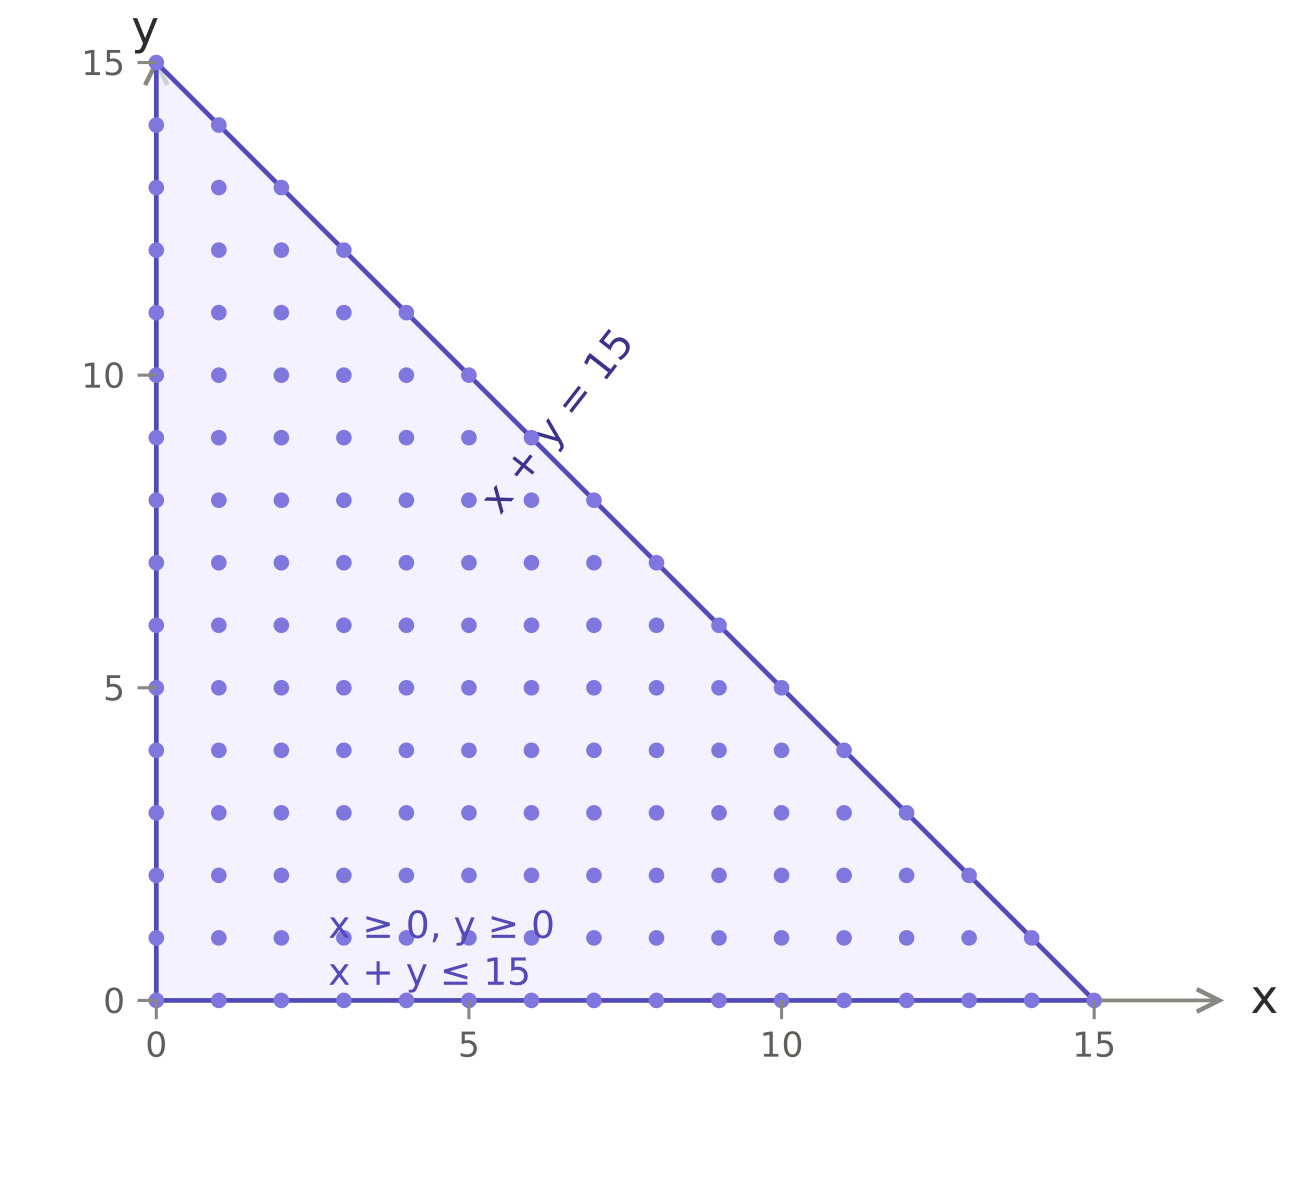
\includegraphics[width=0.6\linewidth]{multinomial_support_region.jpg}
\end{figure}
Independence would require a rectangular support, so $X$ and $y$ are NOT independent.

This is trivial because if $X$ and $Y$ are independent, we have:
$$f(x,y)=f_X(x)f_Y(y)$$
So $f_X(x)>0,f_Y(y)>0$ implies $f(x,y)>0$, this forces the set of points to be the Cartesian product of $X$ and $Y$, the region must be rectangular. (However, in this problem, $(x,y)=(15,15)$, $f(x,y)\ne f_X(x)f_Y(y)$ obviously)
\subsection*{(c)}
\begin{align*}
    P(X=10,Y=4)&=f(10,4) \\
    &=\frac{15!}{10!4!1!}\cdot(0.6)^{10}\cdot(0.3)^4\cdot(0.1)^1 \\
    &=0.0735
\end{align*}
\subsection*{(d)}
We should sum over all possible $y$, but we each item is "good" with probability $6/10$, regardless of other categories. So we can view it as the binomial distribution of $n=15$ and $p=\frac{6}{10}$ (where $p$ is the probability of having "good" item)

Thus, the marginal pmf of $X$ is:
$$f_X(x)=P(X=x)=\binom{15}{x}(0.6)^x(0.4)^{15-x}$$
\subsection*{(e)}
\begin{align*}
    P(X\le 11)&=1-P(X>11) \\
    &=1-(P(X=12)+P(X=13)+P(X=14)+P(X=15)) \\
    &=1-(\binom{15}{12}(0.6)^{12}(0.4)^3+\binom{15}{13}(0.6)^{13}(0.4)^2+\binom{15}{14}(0.6)^{14}(0.4)^1+\binom{15}{15}(0.6)^{15}) \\
    &=0.9095
\end{align*}

\newpage{}
\section*{4.2-3}
\noindent\makebox[\linewidth]{\rule{\linewidth}{0.4pt}}
\begin{theorem}
The expected values of two random variables is multiplicative if \textbf{they are indenpendent}, i.e., $E[XY]=E[X][Y]$
\end{theorem}
\begin{proof}
If $X$ and $Y$ are independent (and $\mathcal{X}$ and $\mathcal{Y}$ are the sample spaces for $X$ and $Y$ respectively.), it holds that

\begin{equation}
p(x, y) = p(x)p(y) \quad \text{for all} \quad x \in \mathcal{X}, y \in \mathcal{Y} .
\end{equation}

Applying this to the expected value for discrete random variables, we have

\begin{align*}
\text{E}(XY) &= \sum_{x \in \mathcal{X}} \sum_{y \in \mathcal{Y}} (x \cdot y) \cdot f_{X,Y}(x, y) \\ 
&= \sum_{x \in \mathcal{X}} \sum_{y \in \mathcal{Y}} (x \cdot y) \cdot (f_X(x) \cdot f_Y(y)) \\ 
&= \sum_{x \in \mathcal{X}} x \cdot f_X(x) \sum_{y \in \mathcal{Y}} y \cdot f_Y(y) \\ 
&= \sum_{x \in \mathcal{X}} x \cdot f_X(x) \cdot \text{E}(Y) \\ 
&= \text{E}(X)\text{E}(Y) . 
\end{align*}

And applying it to the expected value for continuous random variables, we have

\begin{align*} 
\text{E}(XY) &= \int_{\mathcal{X}} \int_{\mathcal{Y}} (x \cdot y) \cdot f_{X,Y}(x, y) \,dy \,dx \\ 
&= \int_{\mathcal{X}} \int_{\mathcal{Y}} (x \cdot y) \cdot (f_X(x) \cdot f_Y(y)) \,dy \,dx \\ 
&= \int_{\mathcal{X}} x \cdot f_X(x) \int_{\mathcal{Y}} y \cdot f_Y(y) \,dy \,dx \\ 
&= \int_{\mathcal{X}} x \cdot f_X(x) \cdot \text{E}(Y) \,dx \\ 
&= \text{E}(X)\text{E}(Y) . 
\end{align*}
\end{proof}

\begin{theorem}
    Suppose $X$ and $Y$ are two random variables, then:
    $$\mathrm{Var}(X+Y)=\mathrm{Var}(X)+\mathrm{Var}(Y)+2\mathrm{Cov}(X,Y)$$
\end{theorem}
\begin{proof}
We can follow the definition of variance and covariance, and writes:
\begin{align*}
    \mathrm{Var}(X+Y)&=E[(X+Y-\mu_{X+Y})^2] \\
    &=E[[(X-\mu_X)+(Y-\mu_Y)]^2] \\
    &=E[(X-\mu_X)^2]+E[(Y-\mu_Y)^2]+2E[(X-\mu_X)(Y-\mu_Y)] \\
    &=\mathrm{Var}(X)+\mathrm{Var}(Y)+2\mathrm{Cov}(X,Y)
\end{align*}
The proof is completed here.
\end{proof}
\begin{theorem}
    Suppose $X$ and $Y$ are two independent random variables, then $\mathrm{Cov}(X,Y)=0$.
\end{theorem}
\begin{proof}
By the formula of covariance and theorem 0.1, we have:
$$Cov(X,Y)=E[XY]-E[X]E[Y]=E[X]\cdot E[Y]-E[X]\cdot E[Y]=0$$
\end{proof}
\noindent\makebox[\linewidth]{\rule{\linewidth}{0.4pt}}
\subsection*{(a)}
Let $Z$ be the outcome of the second roll:
$$\mu_X=E[X]=\mu_Z=E[Z]=\frac{1+2+3+4}{4}=2.5$$
Since $Y=X+Z$:
$$\mu_Y=E[Y]=E[X+Z]=E[X]+E[Z]=5$$
Then we can calculate $\sigma_X^2$ and $\sigma_Y^2$:
\begin{align*}
    \sigma_X^2&=E[X^2]-(E[X])^2 \\
    &=\sum^4_{k=1}k^2/4-(2.5)^2 \\
    &=1.25 \\
    \sigma_Y^2&=\sigma_X^2+\sigma_Z^2+2\mathrm{Cov}(X,Z) \\
    &=\sigma_X^2+\sigma_Z^2=1.25+1.25=2.5
\end{align*}
The last equation comes from theorem 0.2.

Finally, we can calculate the covariance between $X$ and $Y$ using the following steps:
\begin{align*}
    \mathrm{Cov}(X,Y)&=\mathrm{Cov}(X,X+Z) \\
    &=E[X(X+Z)]-E[X]E[X+Z] \\
    &=E[X^2]+E[XZ]-(E[X])^2-E[X]E[Z] \\
    &=E[X^2]-(E[X])^2+E[XZ]-E[X][Z] \\
    &=\sigma_X^2+0=1.25 \\
    \rho&=\frac{\mathrm{Cov}(X,Y)}{\sigma_X\sigma_Y} \\
    &=\frac{1.25}{\sqrt{1.25}\sqrt{2.5}}\\
    &=0.7071
\end{align*}

\subsection*{(b)}
Suppose the regression line is $y=mx+c$, then slope $m$ and intercept $c$ are:
\begin{align*}
    m=\rho\cdot\frac{\sigma_Y}{\sigma_X}=0.7071\cdot\frac{\sqrt{2.5}}{\sqrt{1.25}}\approx 1 \\
    c=\mu_Y-\mu_X=2.5
\end{align*}
Hence, the line is $y=x+2.5$. It's very intuitive because the regression line is exactly taking the first roll ($X$), then add the average of the second roll ($Z$ with $E[Z]=2.5$).

\begin{figure}[H]
    \centering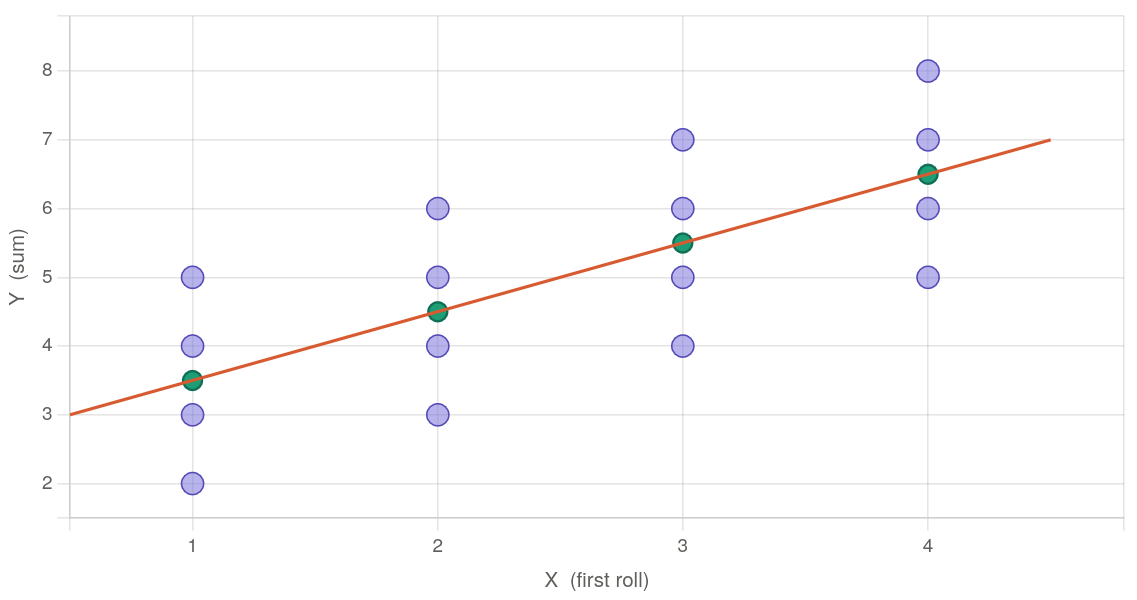
\includegraphics[width=0.9\linewidth]{canvas.png}
    \caption{The least square regression line ($y=x+2.5$)}
\end{figure}
The purple dots are all the possible outcomes. The green dots show the conditional means $E[Y | X = x] = x + 2.5$ for each $x$, and the regression line (The red line) passes exactly through all four of them, this is a beautiful confirmation that the line $\hat{y} = x + 2.5$ is correct

\end{document}
% how to display codes?
% \begin{minted}[frame=lines,framesep=2mm,baselinestretch=1.2,linenos,breaklines]{python}
% \end{minted}

% how to display images?
% \begin{figure}[H]
%     \centering
%     \includegraphics[width=0.5\linewidth]{}
%     \caption{Caption}
% \end{figure}
% test
